\chapter{Fluidos}


\noindent El estudio de los fluidos es de vital importancia, dado que en la actualidad se tienen aplicaciones industriales y tecnológicas con un gran impacto social. Son sustancias con características muy particulares, cuando se utiliza la expresión fluido se refiere a líquidos y gases, además dada su composición molecular se consideran como un medio continuo, esto quiere decir que para el estudio de la dinámica del sistema se consideran volúmenes diferenciales que son pequeños respecto del fluido macroscópico pero grandes en relación con las distancias intermoleculares de la sustancia.

\medskip

\noindent La descripción matemática de un fluido se hace a través de un campo vectorial de velocidades $v = v(x,y,z,t)$ que se supone una función finita y continua en las variables espaciales, para asegurar esto se exige que las primeras derivadas sean continuas en todo el dominio para verificar que las funciones estén representando correctamente la física del campo continuo. Es importante mencionar que la velocidad descrita del fluido es la que pasa por puntos fijos definidos $(x,y,z)$ en un tiempo $t$ determinado, la descripción se hace con puntos fijos tal y como lo propone un sistema de coordenadas Euleriano y no siguiendo el punto material asociado con  partículas fijas dentro del fluido tal y como lo hace la descripción Lagrangiana. Tres campos escalares correspondientes a las magnitudes termodinámicas. La primera de ellas es la presión $p = p(x,y,z,t)$ que caracteriza la fuerza interna (stress) que  representa la fuerza por unidad de área, que por definición es una cantidad macroscópica, por otra parte se considera la  Temperatura $T = T(x,y,z,t)$ esta cantidad recopila todos los aportes de energía cinética que en promedio tienen las partículas dentro del fluido, por último se considera la densidad $\rho = \rho(x,y,z,t)$ que da cuenta de como se distribuyen a lo largo del espacio las partículas de fluido. Estas tres cantidades determinan el estado del sistema, en el caso ideal se utiliza la ecuación de estado de gases ideales , dicha ecuación propone una relación entre las cantidades escalares propuestas anteriormente para poder estudiar y predecir efectivamente el comportamiento del sistema, en general esta ecuación de estado es desconocida y por lo regular se debe teorizar para poder describir teóricamente el comportamiento general del sistema. Apartir de este punto se empieza el camino para encontrar las ecuaciones que describen la dinámica de un fluido.




\section{Ecuaciones de Navier-Stokes}

\noindent Un Fluido es un medio continuo en el espacio, tal medio se piensa como una composición de pequeñas partículas puntuales. La mecánica clásica es una rama de la física que intenta describir el comportamiento de los cuerpos ya sean sólidos, líquidos o gaseosos. Construye su formalismo matemático entre la experimentación y la teoría, en los fluidos se trata de construir un teoría que sirva de modelo a un subconjunto de fenómenos reales, por la naturaleza de modelo renuncia a la pretensión de la exactitud en la descripción y parte del hecho de reflejar y permitirnos intuir la realidad física subyacente. 
\medskip

\noindent Los fluidos en primera aproximación están descritos por la ecuación de Euler , que en resumen es imponer la conservación de la masa, momento y energía en el fluido\cite{Landau}, inicialmente se construye considerando que es un proceso reversible, dado que no se suponen pérdidas de energía\cite{George}, se escribe la ecuación de Euler 

\begin{eqnarray}
\frac{\partial (\rho v_{i})}{\partial t} = -\frac{\partial \Pi_{ik}}{\partial x_{k}}
\end{eqnarray}

\noindent Donde $\Pi_{ik}$ es el tensor de densidad de flujos de impulso, definido de la siguiente manera.

\begin{eqnarray}
\Pi_{ik} = p\delta_{ik} + \rho v_{i}v_{k}
\end{eqnarray}


\noindent Esta cantidad representa una transferencia de momento (proceso  reversible) dado por el transporte mecánico de las partículas de fluido en el espacio. El punto de partida para obtener la dinámica de Navier Stokes será considerar que la viscocidad se debe a una transferencia de momento en donde no se conserva la energía, por tanto se tiene un proceso irreversible , de unos lugares donde la velocidad es grande a otros donde la velocidad es pequeña. Entonces en la definición del tensor de impulsos se adiciona un término que da cuenta de la transferencia de impulso viscoso. Por lo tanto

\begin{eqnarray}
\Pi_{ik} = p\delta_{ik} + \rho v_{i}v_{k} - \sigma^{'}_{ik}=-\sigma_{ik}+\rho v_{i}v_{k}
\end{eqnarray}

\noindent definiendo el tensor de tensiones $\sigma_{ik} $ y análogamente el tensor de tensiones de la viscocidad $\sigma^{'}_{ik}$, se considera que este último expresa la parte de momento que no se transfiere como momento, es decir, solamente por procesos de fricción interna. Para encontrar la forma del tensor de tensiones de la viscosidad se estudia el fundamento de las partículas de fluido. La única manera de que exista rozamiento es asumir que entre las partículas de fluido tienen velocidades diferentes, por lo tanto existe un movimiento relativo de las mismas, entonces se hacen dos aproximaciones; en la primera aproximación, se asume que $\sigma^{'}_{ik}$ depende de las derivadas espaciales de la velocidad, además que solo depende de las primeras derivadas y su relación es lineal, puesto que $\sigma^{'}_{ik}$ debe anularse para $v = \text{cte}$. La segunda condición que se impone es que $\sigma^{'}_{ik}$ debe anularse cuando se tiene rotación uniforme, dado que en tal situación no se produce rozamiento interno en el fluido. El tensor que cumple tales condiciones tiene la forma siguiente

\begin{eqnarray}
\sigma^{'}_{ik} = \eta\left(\frac{\partial v_{i}}{\partial x_{k}} + \frac{\partial v_{k}}{\partial x_{i}} - \frac{2}{3}\delta_{ik}\frac{\partial v_{l}}{\partial x_{l}}\right) + \zeta\delta_{ik}\frac{\partial v_{l}}{\partial x_{l}}
\end{eqnarray}

\noindent  definiendo los coeficientes viscosos $\eta = \eta(T,\rho,P)$ y $\zeta=\zeta(T,\rho,p)$, los fluidos que dependen de manera lineal con el strain \cite{Landau} se denominan fluidos ideales. Entonces la ecuación de movimiento que se tiene es

\begin{eqnarray}
\rho\left(\frac{\partial u_{i}}{\partial t} + u_{k}\frac{\partial}{\partial x_{k}}u_{i}\right) = -\frac{\partial p}{\partial x_{i}} + \frac{\partial \sigma^{'}_{ik}}{\partial x_{k}}
\end{eqnarray}

\noindent por tanto

\begin{eqnarray}
\frac{\partial \sigma^{'}_{ik}}{\partial x_{k}} &=& \eta\left(\frac{\partial^{2} v_{i}}{\partial x_{k}\partial x_{k}}+ \frac{\partial^{2} v_{k}}{\partial x_{k}\partial x_{i}}-\frac{2}{3}\delta_{ik} \frac{\partial^{2} v_{l}}{\partial x_{k} \partial x_{l}}\right)+\zeta \frac{\partial^{2} v_{l}}{\partial x_{k}\partial x_{l}}\nonumber \\
&=&\eta\left(\frac{\partial^{2} v_{i}}{\partial x_{k}\partial x_{k}} + \frac{\partial}{\partial x_{i}}\left(\frac{\partial v_{k}}{\partial x_{k}}\right)-\frac{2}{3}\delta_{ik}\frac{\partial}{\partial x_{k}}\left(\frac{\partial v_{l}}{\partial x_{l}}\right)\right) + \zeta \frac{\partial^{2} v_{l}}{\partial x_{k}\partial x_{l}}\nonumber \\
&=& \eta\left(\frac{\partial^{2} v_{i}}{\partial x_{k}\partial x_{k}}\right) + \frac{1}{3}\eta\frac{\partial}{\partial x_{i}}\left(\frac{\partial v_{l}}{\partial x_{l}}\right)+ \zeta \frac{\partial^{2} v_{l}}{\partial x_{k}\partial x_{l}}\nonumber \\
&=& \eta\frac{\partial^{2} v_{i}}{\partial x_{k}\partial x_{k}} + \left(\zeta + \frac{1}{3}\eta\right)\frac{\partial}{\partial x_{i}}\frac{\partial v_{l}}{\partial x_{l}}
\end{eqnarray}


\noindent la ecuación que describe un fluido en general está dada por 

\begin{eqnarray}
\rho\left(\frac{\partial u_{i}}{\partial t} + u_{k}\frac{\partial}{\partial x_{k}}u_{i}\right) = -\frac{\partial p}{\partial x_{i}} + \eta\frac{\partial^{2} v_{i}}{\partial x_{k}\partial x_{k}} + \left(\zeta + \frac{1}{3}\eta\right)\frac{\partial}{\partial x_{i}}\frac{\partial v_{l}}{\partial x_{l}}
\end{eqnarray}


\noindent que de forma vectorial se escribe de la siguiente forma

\begin{eqnarray}
\rho \left(\frac{\partial \vec{v}}{\partial t}+(\vec{v} \cdot \nabla )\vec{v}\right) = -\nabla p +\eta \nabla^{2}\vec{v} + \left(\zeta + \frac{1}{3}\eta\right)\nabla(\nabla \cdot \vec{v}) 
\end{eqnarray}

\noindent cuando el fluido se considera incompresible se asume a priori el hecho de $\nabla \cdot \vec{v} = 0$

\begin{eqnarray}
\label{NS}
\frac{\partial \vec{v}}{\partial t}+(\vec{v} \cdot \nabla )\vec{v} = -\frac{1}{\rho}\nabla p +\frac{\eta}{\rho} \nabla^{2}\vec{v}
\end{eqnarray}

\noindent que es la ecuación de Navier Stokes en donde el tensor de tensiones en un fluido incompresible está dado por 

\begin{eqnarray}
\sigma_{ik} = -p\delta_{ik} + \eta\left(\frac{\partial v_{i}}{\partial x_{k}} + \frac{\partial v_{k}}{\partial x_{i}  }\right)
\end{eqnarray}.

\noindent La viscosidad de un fluido incompresible queda determinada por el coeficiente $\eta$ (viscosidad dinámica).Por último se escriben las ecuaciones de Navier Stokes en términos de ecuaciones de conservación y presentan la siguiente forma 

\begin{eqnarray}
\label{continuidad}
\frac{\partial \rho}{\partial t}+\frac{\partial }{\partial x_{k}}(\rho u_{k})&=& 0 \qquad \\
\label{NS}
\frac{\partial(\rho u_{i})}{\partial t}+\frac{\partial}{\partial x_{k}}(\rho u_{k}u_{i})&=&-\frac{\partial p}{\partial x_{i}}+\frac{\partial \sigma_{ij}}{\partial x_{j}} \qquad 
\end{eqnarray}

\section{Turbulencia}

\noindent Cuando se estudian las ecuaciones  Navier Stokes se intenta dar una descripción matemática y modelar el movimiento de los fluidos bajo ciertas simplificaciones, sin embargo en la naturaleza se presentan muchas más interacciones que se deben tener en cuenta a la hora de esta tarea. El objetivo que se persigue será el de encontrar un función matemática que describa completamente un sistema físico , esta solución requiere estabilidad y exactitud para poder considerarla como provechosa y utilizarla en aplicaciones concretas, a partir de este punto se encuentra con el concepto de turbulencia. En nuestro entorno cotidiano se encuentran muchos ejemplos familiares del comportamiento turbulento, la interacción de nubes en el cielo, flujo en tuberías en aplicaciones de ingeniería, mezcla de sustancias en procesos químicos, flujo de aire a través de carros, submarinos y aviones, la fotosfera solar y muchos ejemplos interesantes. El estudio y descripción de la turbulencia se presenta entonces como una actividad interdisciplinaria la cual tiene un rango muy amplio de aplicaciones, dado que no se tiene un modelo matemático formal para atacar y encontrar soluciones se utiliza la estadística para afrontar este problema, por tal razón una de las características es la aleatoriedad en tanto nuestros análisis se basan en métodos estadísticos. 

\medskip

\noindent La turbulencia causa un mezclado rápido e incrementa la tasa de transferencia de momento, calor  y masa, de hecho la difusividad es uno de los tópicos más interesantes a la hora de analizar la dinámica del sistema, estos comportamientos aparecen siempre con altos números de Reynolds entonces vemos que las inestabilidades se originan en la interacción de los términos viscosos y la no linenalidad en los términos inerciales en las ecuaciones de movimiento \eqref{NS}, esta interacción es muy compleja dado que las matemáticas de las ecuaciones diferenciales parciales y no lineales no tiene soluciones concretas actualmente, aún no se tienen herramientas poderosas para atacar el problema, de hecho podemos mencionar que es uno de los problemas actuales sin resolver en la física. La consecuencia física más importante es entender de mejor manera los procesos de transporte en los fluidos, este fenómeno describe muchas sub estructuras relacionadas con el transporte de cantidades físicas asociadas, aparentemente, con procesos aleatorios e inestabilidades a pequeña escala. 


\subsection{Finite-Mode Model}

\noindent En orden de entender la naturaleza  'aleatoria' de las soluciones a ecuaciones diferenciales se estudia un modelo que evidencia la estructura de la turbulencia.

\medskip

\noindent Se considera el siguiente sistema de ecuaciones diferenciales

\begin{eqnarray}
\frac{dx_{i}}{dt} = x_{i+1}x_{i+2}+x_{i-1}x_{i-2}-2x_{i+1}x_{i-1}\quad (i =1,\cdots,5)\qquad x_{i} = x_{i+5}
\end{eqnarray}.

\noindent El sistema se considera análogo a las ecuaciones de Navier-Stokes que describen un fluido inviscido respecto de tres ideas fundamentales. 

\begin{itemize}
    \item Involucra interacciones cuadráticas en sus grados de libertad , tal y como lo hace en el termino convectivo la ecuación \eqref{NS}
    
    \item La energía se conserva , en el sentido 
    
    \begin{eqnarray}
    \frac{d}{dt}\left(\frac{1}{2}\sum_{i=1}^{5}x_{i}^{2}\right) = 0
    \end{eqnarray}
    
    Toda la evolución de las trayectorias de las coordenadas $x_{i}(t)$se da en una esfera de cinco dimensiones $\sum x_{i}^{2}=cte$ en el espacio de fase
    
    \item El teorema de Liouville es válido
    
    \begin{eqnarray}
    \sum_{i=1}^{5}\frac{\partial}{\partial x_{i}}\left(\frac{dx_{i}}{dt}\right) = 0
    \end{eqnarray}
    
    cuando esta condición se cumple el ensamble en el espacio de fase de cinco dimensiones preserva el volumen, manteniendo una mecánica estadística del equilibrio
    
\end{itemize}


\noindent Entonces el espacio de fase está dado por cinco coordenadas y cinco momentos canónicamente conjugados $(x_{1},x_{2},x_{3},x_{4},x_{5})$, en donde el estado del sistema esta representado por un punto en este espacio y la evolución en el tiempo será la trayectoria. 

\begin{figure}[H]
\centering
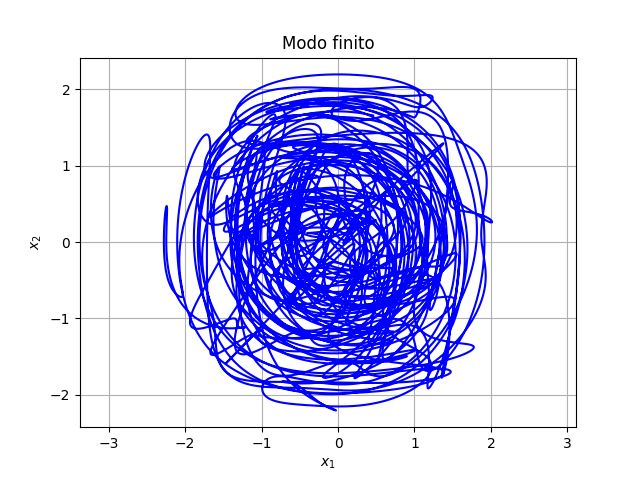
\includegraphics[scale =0.8]{FiniteMode1.png}
\caption{Plot de la trayectoria en el espacio de fase de las coordenadas $x_{1}$ y $x_{2}$ para un tiempo de $0<t<200$ con condiciones iniciales 
$x_{1}(0) = 0540323$, $x_{2}(0) = -1.543569$ ,$x_{3}(0) = -0.680421$ ,$x_{4}(0) = -1.185361$ ,$x_{5}(0) = -0.676307$
estas trayectorias se determinaron numéricamente con un esquema Euler hacia adelante  de primer orden (El desarrollo del esquema numérico se puede encontrar en Github siguiendo este  \href{https://github.com/GoSAUN/Hartmann/tree/master/Codes/FiniteMode}{link})}
\label{FiniteModel}
\end{figure}

\noindent Se puede ver que cada punto en el espacio de fase es inestable, en este caso el sistema es fuertemente mezclado, por tanto preserva la hipótesis de ergodicidad dada por el Teorema de Birkoff, esto significa que cada estado en el espacio de fase dura , en promedio, la misma cantidad de tiempo en todo los lugares del volumen en este espacio. Esto es de gran ayuda dado que el estudio de una sola órbita da una idea general del sistema para cualquier trayectoria.

\subsection{Problemas con las ecuaciones de Navier Stokes}

\noindent Las ecuaciones de Navier Stokes estudiadas en la sección anterior \eqref{NS}  son el punto de partida para el estudio de la turbulencia. Se sabe que en principio no se tiene una ecuación de estado para poder tener completo el sistema de ecuaciones diferenciales, sin embargo el campo de presiones no satisface ninguna ecuación solamente sirve como una condición para preservar la condición de incompresibilidad para cualquier tiempo, Tomando la divergencia de \eqref{NS}, se tiene 

\begin{eqnarray}
\frac{\partial p}{\partial x_{i}\partial x_{i}} = -\frac{\partial}{\partial x_{i}}\left(u_{k}\frac{\partial u_{i}}{\partial x_{k}}\right)
\end{eqnarray}

\noindent entonces la presión es determinada a cada instante de tiempo por el campo global de velocidades, solucionando una ecuación de Poisson, teniendo en cuenta que el efecto instantáneo de las regiones distantes en el flujo local a través de la presión se dan solamente en el límite de la velocidad Mach cero, o de manera equivalente a una velocidad del sonido en el fluido infinita. Se puede ver el siguiente manejo algebraico de las ecuaciones de NAvier Stokes incompresibles para entender mejor la anterior idea

\begin{eqnarray}
\frac{d}{dt}\frac{1}{2}\int_{V}|v|^{2}d\vec{x} = -\nu\int_{V}\frac{\partial u_{\alpha}}{\partial x_{\beta}\partial x_{\beta}}d\vec{x}  
\end{eqnarray}

\noindent donde $V$ es el volumen ocupado para el fluido. Esta relación se relaciona con el balance energético global en el fluido, se puede ver que el término convectivo $u_{k}\frac{\partial u_{i}}{\partial x_{k}}$ y el término de presión $\frac{\partial p}{\partial x_{i}}$  de manera separa conservan la energía total, mientras que el termino viscoso disipa energía en cuanto $\nu > 0$. La anterior ecuación evidencia que todos lo movimientos en una dominio finito debe cesar cuando $t\rightarrow\infty$ siempre y cuando no exista fuerzas externas. 

\noindent Las matemáticas para afrontar las ecuaciones de Navier-Stokes no están desarrolladas completamente, dado que no existe una solución general ni única. Por ahora so se puede trabajar sobre  la extrema simplificación que se hace al trabajar en fluidos ideales. Se plantea el sistema de estudio en un espacio infinito y sujetas a condiciones de decaimiento rápido en las condiciones iniciales 
\begin{eqnarray}
\label{regularidad}
\left|\frac{\partial^{\alpha}u_{o,t}}{\partial x}\right| &\leq& C_{\alpha,K}(1+|x|)^{K}, \qquad \forall \alpha, \ \forall K\\
\left|\frac{\partial^{\alpha}}{\partial x}\frac{\partial^{m}}{\partial t}\vec{F}(\vec{r})\right| &\leq& C_{\alpha,m,K}(1+|x|+t)^{K}, \qquad \forall \alpha, \ ,\forall \beta \forall K
\end{eqnarray}

\noindent y se consideran admisibles las soluciones clásicas de $\vec{u},p,\rho\in C^{\infty}(\rm I\!R\times(0,T))$ que cumplen 

\begin{eqnarray}
\int u^{2}(\vec{r},t)d\vec{r} < \infty\qquad \forall t
\end{eqnarray}

\noindent Esto sugiere que en todo el sistema la energía cinética está acotada. En este punto surge un problema de decisión en cuanto a la manera de resolver el sistema de Navier Stokes

\begin{itemize}
    \item \textbf{Problema de existencia y regularidad:} Se elige $\nu > 0$ y no se consideran fuerzas externas, además se supone que las condiciones iniciales cumplen las condiciones de regularidad \eqref{regularidad} , compresibilidad y decrecimiento rápido en el infinito. Demostrar que existe $\vec{u},\rho\in C^{\infty}(\rm I\!R^{n}\times(0,\infty))$, con energía cinética finita , que resuelve el sistema de ecuaciones de Navier-Stokes en el sentido clásico y $\vec{u}$ y toma el valor de la condición inicial. 
    
    
    
    \item \textbf{Problema colapso de la solución:} Se elige $\nu>0$, encontrando un dato inicial $\vec{u}_{o]}$ y una función que agrupe las fuerzas externas del sistema, tales que no existe una solución clásica de los campos asociados del sistema de ecuaciones de Navier-Stokes 
    
    \item \textbf{Problema de unicidad:} Dada un conjunto de soluciones aceptables físicamente, demostrar que la solución es única durante el tiempo de existencia considerado en el sistema 
    
\end{itemize}

\noindent Se trata entonces principalmente de un problema de decisión tenemos varias opciones. Sí se asume que $T=\infty$ por un tiempo pequeño entonces la solución existe y es regular. Esto fue demostrado por Lery en 1933. Ahora si $\vec{u}_{o}$ es fuertemente oscilante también es regular y existe la solución, sin embargo si el problema del colapso de la solución fuese cierto y una solución no pudiera ser calculada más allá de un tiempo $T>0$, entonces la velocidad se debe hacer infinita cuando $t\rightarrow T$, por tanto es una contrariedad física, dado que la energía sería infinita. Este tópico es un tema de investigación de vanguardia dado que no se tiene unicidad para las soluciones de sistemas físicos que involucren las ecuaciones de Navier-Stokes.

\subsection{Escalas de Turbulencia }

\noindent Se considera un flujo completamente turbulento con un número de Reynolds\footnote{Se recuerda que el número de Reynolds está dado por $R = \frac{\mathcal{U}\mathcal{L}}{\nu}$} alto con una velocidad característica $\mathcal{U}$ y longitud característica $\mathcal{L}$. EL primer concepto que se va a considerar que que la turbulencia puede entenderse como una composición de remolinos con diferentes tamaños.
El tamaño de los remolines está dado por una longitud característica $l_{o}$ la cual es comparable con la escala de fluido $\mathcal{L}$y con una velocidad característica $u(l_{o})$ la cual es comparable con $\mathcal{U}$ ademas con número de Reynolds $Re_{o} = u_{o}l_{o}/\nu$.(que es largo comparado con $Re$).

\medskip

\noindent Richardson fue el primero en proponer la idea de la cascada de energía, esta noción consiste en plantear que los remolinos grandes son inestales y se rompen, transfiriendo energía a remolinos más pequeños. Estos remolinos más pequeños también tienden a romperse y seguir transportando energía a otro mas pequeños aún, esto es el concepto denominado \emph{Cascada de energía}, en la cual la energía se transmite sucesivamente de remolinos grandes a los más pequeños. La tasa de disipación $\varepsilon$ es determinada por el primer proceso en la secuencia de cascada, la cual es del orden $\sim u_{o}^{2}$ y en la escala del tiempo $\sim l_{o}/u_{o}$, entonces la tasa de transferencia de energía se supone como $u_{o}^{2}/\tau = u_{o}^{3}/l_{o}$ independiente de $\nu$ (siempre con la consideración de número de Reynolds alto).

\medskip

\noindent Para empezar a considerar la hipótesis de Kolmogorov empezando por la pregunta ¿Cual es la longitud característica del remolino más pequeño al cual se le tranfiere energía de uno más grande? Como $l_{o}$ decrece, ¿esto hace que $u(l_{o})$ y $\tau(l_{o})$?. Estas preguntas las trató Kolmogorov que respondió a través de tres hipótesis. La primera hipótesis está relacionada con la isotropía de los movimientos de pequeña escala, en general los remolinos grandes son afectados por las condiciones de frontera y son anisotrópicos, Kolmorogov asegura que la anisotropía se pierde en el proceso de reducción de escala entre remolinos grandes a pequeños

\medskip

\hangindent=0.7cm \textbf{Hipótesis de isotropía local: } A un numero de Reynolds Suficientemente alto, las escalas pequeñas en el movimiento turbulento es estadísticamente isotrópico $(l<<l_{o})$

\noindent en este caso se entiende la escala pequeña bajo la definición $l_{p} \approx (1/6)l_{o}$ \cite{pope}\footnote{Justo acá se hace la deducción de este criterio utillizando el tensor del espectro de la velocidad} como el límite entre las escalas grandes donde se tiene anisotropía en los remolinos y las pequeñas donde se tiene isotropía. Kolmogorov argumenta que las esclas grandes pierden energía pasando está a manera de cascada hacia escalas más bajas, la información sobre la geometría de los grandes remolinos se determina por el campo de velocidades y las condiciones de frontera. 

\medskip

\hangindent=0.7cm \textbf{Primera hipótesis de similaridad de Kolmogorov: }En cada flujo turbulento con un número de Reynolds suficientemente alto , la estadística del movimiento de las pequeñas escalas tiene una forma universal única determinada por $\nu$ y $\varepsilon$

\medskip

\noindent El rango de longitud $l<l_{p}$ está relacionado con una categoría de equilibrio universal, en tal rango las escalas de tiempo del fluido, caracterizadas por $l/u(l)$, son pequeñas comparadas con $l/u_{o}$, de tal manera que los pequeños remolinos se adaptan rápidamente para mantener el equilibrio en la transferencia de energía desde las escalas más altas. Dados los dos parámetros $\varepsilon$ y $\nu$  existen unos parámetros únicos de longitud, velocidad y tiempo que pueden ser formados. Estos son

\begin{eqnarray}
\eta &=& \left(\frac{\nu^{3}}{\varepsilon}\right)^{1/4}\\
u_{\eta} &=& (\varepsilon\nu)^{1/4}\\
\tau_{\eta}&=&\left(\frac{\nu}{\varepsilon}\right)^{1/2}
\end{eqnarray}

\noindent dos identidades provenientes de la definiciones anteriores indican que las escalas de Kolmogorov se caracterizan por ser muy pequeñas. El número de Reynolds basado en las escalas de Kolmogorov se define como la unidad, es decir, $\eta u){\eta}\nu=1$, que es consistente con la noción de cascada . Por tanto la la tasa de disipación está dada por 

\begin{eqnarray}
\varepsilon = \nu\left(u_{\eta}\eta\right)^{2}=\frac{\nu}{\tau_{\eta}^{2}}
\end{eqnarray}

\noindent se evidencia que $(u_{\eta}/\eta)=1$. Las relaciones de las escalas pequeñas y grandes están determinadas por las siguientes definiciones , utilizando el hecho $\varepsilon \sim u_{o}^{3}/l_{o}$

\begin{eqnarray}
\frac{\eta}{l_{o}}\sim Re^{-3/4},\qquad \frac{u_{\eta}}{u_{o}}\sim Re^{-1/4},\qquad
\frac{\tau_{\eta}}{\tau_{o}}\sim Re^{-1/2}
\end{eqnarray}

\noindent entonces se ve que para números de Reynolds altos , las velocidades y tiempo de los remolinos pequeños $u_{\eta}$, $\tau_{\eta}$ son chicos en comparación con los grandes, caracterizados por $u_{o}$ y $\tau_{o}$.

\medskip

\hangindent=0.7cm \textbf{Segunda hipótesis de similaridad de Kolmogorov: }En cada flujo turbulento con un número de Reynolds suficientemente alto ,la estadística del movimiento de escala $l$ en el rango  $l_{o}\gg l \gg\eta$ tiene una forma universal que es determinada unicamente por $\varepsilon$ in tependiente de $\nu$

\medskip

\noindent De igual manera que en el anterior análisis de la primera hipótesis de Kolmogorov se define una longitud de escala dada por $l_{d} = 60\eta$, entonces se trabajara bajo la siguiente región $l_{p}>l>l_{d}$. Esta longitu de escala $l_{d}$ ...





\subsection{El espectro de energía}


\noindent Queda por estar determinado como la energía cinética turbulenta está distribuida en los remolinos de diferentes tamaños. Considerando una turbulencia homogénea y considerando un función del espectro de energía $E(k)$, la dinámica del movimiento se caracteriza por el número de onda  $k=2\pi/l$ y el rango de números de onda en el cual el sistema se encuentra 

\begin{eqnarray}
\varepsilon_{(k_{a},k_{b})} = \int_{k_{a}}^{k_{b}}E(k)dk
\end{eqnarray}

\noindent A partir de esta integral se puede encontrar la tasa de disipación \cite{pope} $\varepsilon$ para el movimiento en el rango de numero de onda $(k_{a},k_{b})$, y está dada por 

\begin{eqnarray}
\varepsilon_{(k_{a},k_{b})} = \int_{k_{a}}^{k_{b}}2\nu k^{2}E(k)dk
\end{eqnarray}

\noindent Se considera entonces que la función del espectro de energía  cumple una ley de otencias dada de la siguiente manera

\begin{eqnarray}
E(k) = Ak^{-p}
\end{eqnarray}

\noindent donde $A$ y $p$ son constantes. La energía contenida en los número de onda mayor a $k$ son 

\begin{eqnarray}
k_{k,\infty} = \int_{k}^{\infty}E(k')dk' =\frac{A}{p-1}k^{-(p-1)}
\end{eqnarray}

\noindent para el caso de $p>1$ la integral converge, mientras que para $p<1$ diverge. De manera análoga se tiene para la disipación 

\begin{eqnarray}
\varepsilon_{(0,k)}= \int_{0}^{k}2\nu (k')^{2}E(k')dk'=\frac{2\nu A}{3-p}k^{3-p}
\end{eqnarray}

\noindent para $p<3$, pero la integral diverge para valores $p\geq 3$, entonces , p = 5/3 corresponde al espectro de Kolmogorov para el cual las dos integrales convergen. La cantidad de energía en los altos números de onda decrece como $k\sim k^{-2/3}$ a medida que $k$ aumenta, por otra parte la disipación en los número de onda bajos decrese como $\varepsilon \sim k^{-4/3}$ mientras que k va hacia cero. La primera hipótesis de similaridad de Kolmogorov asegura que $k>k_{p} = 2\pi/l_{p}$. Para la segunda hipótesis se tiene que el espectro de energía es

\begin{eqnarray}
E(k) = C\varepsilon^{2/3}k^{-5/3}
\end{eqnarray}

\noindent donde $C$ es una constante universal


